
\documentclass[a4paper,12pt]{article}
\frenchspacing
\usepackage{microtype}
\usepackage{graphicx}
\usepackage{placeins}
\graphicspath{ {./images/} }
\usepackage[pdfauthor={Jenny Vermeltfoort},pdftitle={Model based consistency of variable names for improved high-level understanding.}]{hyperref}

\begin{document}

\title{Model based consistency of variable names for improved high-level understanding.}
\author{Jenny Vermeltfoort}
\date{\today}
\maketitle

\section{Introduction}
While software is written to be interpreted by computers it is of key importance that humans are able to quickly understand it fully. The naming of identifiers is an important tools for software engineers to meaningfully transfer concepts to their colleagues, who might be maintaining, updating or refracturing the code. Comprehensibility of these concepts might be restricted by the innate free characteristics of naming conventions within software languages. It is therefore of interest to identify what kind of identifiers are difficult to interpret and whether formal rules may be developed to create a more structured way of transferring concepts.

This report evaluates two research papers that address these issues. The first, written by Floarian Deissenboeck and Markus Pizka, tries to define a formal model to create conise and consistent naming schemas in their paper \textit{Concise and consistent naming}. The second, \textit{Improving Semantic Consistency of Variable Names with Use-Flow Graph Analysis} written by Yusuke Shinyama, Yoshitaka Arahori, and Katsuhiko Gondow builds a probabilistic model to test if a variable name reflects its intended usage pattern. This report summarizes, and produces a compounded conclusion of both papers. At the end of the report a short paragraph describes the approach used for writing this report.

\newpage
\section{Concise and consistent naming}
Floarian Deissenboeck et al. preamble their paper by describing why bad naming of identifiers is detremental to the quality of software. Software engineers are constantly trying to interpreting identifier and the concepts they represent. It is therefore important that identifiers meaningfully represent a concept. Identifiers are arbitrarily chosen and the developers often lack a broad understanding of the code base as a whole. When a system evolves, concepts might change or become abandoned and often names are not adapted properly. These problems damage the coherence of a project and decrades the quality of the code.

According to the authors, meaningfullness does not properly describe why a variable name is good or bad. They partition the evaluation of a variable name's meaning into two categories, consistency and conciseness. A variable name is consistent when its name only describes one specific concept. When the name is either homonynous or synonymous to multiple concepts it fails this criteria. The word break could mean taking a break or could mean breaking a stick. The word break thus requires contextualization to fully understand it. Conciseness is determined by the exactness in which a name describes a concept. A example is a hyponym. The word red is a hyponym of the word color, therefore red describes a object more exact then the word color does. The sentence "the colorfull balloon" is more cryptic then the sentence "the red balloon".

Most identifiers within the software language are verb-noun compounds, thus identifiers commonly specialized concepts. The variable \textit{BinaryNodeTree} is a specialized \textit{NodeTree} which in turn is a specialized \textit{Tree}. Two types of compounds are described in the paper, endrocentric and exocentric. Endrocentric is when a compound is made up of a main and a modifier concept. \textit{School dairy} is a special kind of dairy. Exocentric means that no main concept exists within a compound; is a \textit{television painting} a television or a painting? The authors find that endocentric are the easiest to understand and are therefore the only compound that may exist in the software language.

Analysis on the code base of \textit{Eclipse} show that the source code is made up of 142.275 different identifiers and 11.482 different atomic words; also atomic words are often written in different manners (\textit{frag, fragment, fragments, etc}). According to Deissenboeck et al. this is detremental to the coheresion of the project. Analysis of the project \textit{CloneDetective} shows that code decay occured since many identifiers where not adapted after code refracturing and as a result some identifiers do not represent their correct concepts. Analysis of more projects show simular results.

The authors have developed a half automated tool for Java developers. The tool, a plugin for Eclips IDE, is a identifier dictionary which presents popups and allows autocompletion when creating variable names. It also is capable of automated refacturing of already existing code. The tool lessens efforts needed to comply with naming rules. The authors seem interested to see how their model works for other mid to large scale code bases.

\newpage

\section{Imrpoving Semantic Consistency}
Yusuke Shinyama et al. find that the semantic consistency of variable names in a code base is an important factor for a high level understanding. In their paper they define an automated method to identify and correct name inconsistency’s over a project. The method is based upon a multitude of research papers; which, in short, conclude that long descriptive names improve understanding and that inconsistent naming results in a decay of code quality.

A multitude of researchers have grasped at the problem of identifying concistency of identifier. One converts source code in word embeddings and relates it to the natural language, another uses manually crafted rules to detect naming bugs, and another validates whether method names properly describe the method’s code contents. Shinyama et al. use a novel approach by trying to identify semantic inconsistency of variable names by comparing the relation of the variable names to its context. Not only looking at method names but also variable names, which accordingly, better infer the project’s meaning and highlevel design.

The consistency of a identifier may be determined by placing the variable name within its context. Code implements a set of operations on a variable, this set of operations is considered the context of a variable name; it is the relation of the name towards its usage. A concrete relationship for every variable name towards its concept is establisched. Then through comparison the concistency of each identifier may be predicted. 

For illustration purposes see the example of a variable name and its context below. The variable name “year\_birth” may be substituted by an arbitrary name “x”. The initial assignment using the method call get\_time\_person and the designation method call calc\_age form the context for variable "x". The last two lines of the example thus define the relation of the variable “x” to its context. By comparing all the variable names that fit this exact relation, consistency may be determined for any variable within the project.

\begin{verbatim}
    int year_birth = get_time_person(person).year;
    int age = calc_age(year_now, year_birth);

    int x = get_time_person(person).year;
    int age = calc_age(year_now, x);
\end{verbatim}

To support automation of this process the paper proposes a graph structure -- a “Use-Flow Graph” (UFG) -- to describe the context of a variable. See the figure below. The graph depicts the origin, the operations and the designation of the variable. By traversing the lanes from top to bottom for each variable an usage pattern is constructed. This usage pattern is the relation of the variable name towards its context, which as described in the paragraphs before may be used for consistency analysis. Certain software specific operations, in this example the mathematical operators, are depicted using unique blocks; think of \textit{while}- and \textit{for}-loops, \textit{if}-statements, and method calls. 

\begin{figure}[ht]
    \centering
    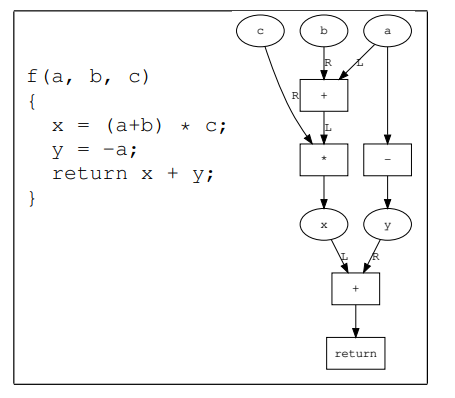
\includegraphics[width=0.7\linewidth]{ufg}
    \caption{example UFG.}
    \label{fig:ufg}
\end{figure}
\hfill
\FloatBarrier

    
The paper shows that the automated method defined by the paper is capable of providing improved consistent naming schemas within a project. However, the authors note a clause concerning the results; the small pool of nine reviewers might be biased which could have skewed the results; also the method is only designed for Java code and software languages with dynamic dispatch and variable aliasing exceed the model's limitations.

\section{Conclusion}
The paper written by Deissenboeck et al. is based on the conclusion made by Schneider that states that meaningfull names are an important factor for better understanding of complex systems. Deissenboeck et al. expand this conclusion by interpolating the word meaningfull over a couple of concrete rules. These rules constitute their model. The paper however solely show the model being used for analysis and does not present any arguments that are based on a statistical fact. It is therefore unknown whether their model acctually improved the understanding of any of these projects.

Both papers seem to agree that the consistency of a variable names depends on its usage pattern; a variable has to correctly describe its intented concept. It is interesting to see how each paper tackles the problem of name consistency in a different manner. Deissenboeck et al. have found a more abstract allround method to describe the meaning of a identifier. While Yusuke et al. have made a very specified and consistent way to determine a identifier's correctness by limiting the scope to project based only. This juxtaposition does seem to depict a relative weakness that arises from researching a subjective topic. While some formal rules may improve cohesion of software development overall, it seems almost impossible to define some objective schema that projects a identifiers meaningfullness. Possibly this gap might be bridged by integrating psychological research into future research of this topic.




\section{Assignment approach}
Firstly I analysed the assignment and devloped a high-level plan. This entails that I wrote a small section of the introduction and predefined the sections. 

Secondly I tried to find an academic paper related to the topic. I used a couple of databases, Leiden University Librarie Catalogue and Google Scholar. Found an older paper written by Deissenboeck et al. in 2005, the article itself and a broad selection of Deissenboeck's papars are highly influencial according to Semantic Scholar. The paper written by Yusuke et al. is less influencial, however it is much more recent (2024). Yusuke et al. have all written a plathora of papers related to the topic and their references used within the article are quite influencial. 

Thirthly I read both papers and made notes and highlights along the way. Then I summarized each paper indivually. I struggled with finding the right balance when it came to descriptiveness and conciseness. So I made quick map with short item descriptions for each paper that I wanted to be part of the summarization. It allowed me to keep things comprehensible and logically sequenced. 

Fourthly I wrote the conclusion, which I formulated from some notes that I made while reading. While I was reading I had some doubts about certain arguments and thought of things that where missing. I also thought about how I would tackle the problem.





% the bibliography
\bibliographystyle{plain}
\bibliography{references}

\end{document}

